
%(BEGIN_QUESTION)
% Copyright 2005, Tony R. Kuphaldt, released under the Creative Commons Attribution License (v 1.0)
% This means you may do almost anything with this work of mine, so long as you give me proper credit

Digital computers communicate with external devices through {\it ports}: sets of terminals usually arranged in groups of 4, 8, 16, or more (4 bits = 1 {\it nybble}, 8 bits = 1 {\it byte}, 16 bits = 2 bytes).  These terminals may be set to high or low logic states by writing a program for the computer that sends a numerical value to the port.  For example, here is an illustration of a microcontroller being instructed to send the hexadecimal number {\tt F3} to port A and {\tt 2C} to port B:

$$\includegraphics[width=15.5cm]{i02168x01.eps}$$

Suppose we wished to use the upper four bits of port A (pins 7, 6, 5, and 4) to drive the coils of a stepper motor in this eight-step sequence:

\medskip
\goodbreak
\item{Step $1$:} {\tt 0001}
\item{Step $2$:} {\tt 0011}
\item{Step $3$:} {\tt 0010}
\item{Step $4$:} {\tt 0110}
\item{Step $5$:} {\tt 0100}
\item{Step $6$:} {\tt 1100}
\item{Step $7$:} {\tt 1000}
\item{Step $8$:} {\tt 1001}
\end{itemize}

As each pin goes high, it drives a power MOSFET on, which sends current through that respective coil of the stepper motor.  By following a "shift" sequence as shown, the motor will rotate a small amount for each cycle. 

Write the necessary sequence of numbers to be sent to port A to generate this specific order of bit shifts, in hexadecimal.  Leave the lower four bit of port A all in the low logic state.

\underbar{file i02168}
%(END_QUESTION)





%(BEGIN_ANSWER)

\medskip
\goodbreak
\item{Step $1$:} $10_{16}$
\item{Step $2$:} $30_{16}$
\item{Step $3$:} $20_{16}$
\item{Step $4$:} $60_{16}$
\item{Step $5$:} $40_{16}$
\item{Step $6$:} $\hbox{C}0_{16}$
\item{Step $7$:} $80_{16}$
\item{Step $8$:} $90_{16}$
\end{itemize}

\vskip 10pt

Follow-up question: write the same sequence in decimal rather than hexadecimal:

\medskip
\goodbreak
\item{Step $1$:}
\item{Step $2$:}
\item{Step $3$:}
\item{Step $4$:}
\item{Step $5$:}
\item{Step $6$:}
\item{Step $7$:}
\item{Step $8$:}
\end{itemize}

%(END_ANSWER)





%(BEGIN_NOTES)

Although the root of this question is nothing more than binary-to-hexadecimal conversion, it also introduces students to the concept of controlling bit states in microcomputer ports by writing hex values.  As such, this question is {\it very} practical!

In case students ask, let them know that a dollar sign prefix is sometimes used to denote a hexadecimal number.  Other times, the prefix 0x is used (e.g., \$F3 and 0xF3 mean the same thing).

%INDEX% Electronics review: numeration system conversions
%INDEX% Electronics review: stepper motor

%(END_NOTES)


